\documentclass[svgnames]{beamer}

\usepackage{pri}
\usepackage{alltt}
\usepackage{graphicx}
\usepackage{tikz}
\usepackage{listings}

\graphicspath{{./}{figures/}{figures/08-xml-figs/}} 

\subtitle{Semi-Structured Data : XQuery}

\begin{document}

\maketitle

\begin{frame} \frametitle{Bibliography}

   \begin{block}{}
        \href{http://www.cs.uic.edu/~liub/WebMiningBook.html}{Bing Liu, Web Data Mining: Exploring Hyperlinks, Contents, and
         Usage Data, 2nd edition}. Chapter 9.
    \end{block}

   \begin{block}{}

    \href{http://www.mir2ed.org/}{Ricardo Baeza-Yates,
            Berthier Ribeiro-Neto, Modern Information Retrieval, 2nd
            edtion}. Chapter 13.

    \end{block}

   \begin{block}{}

    \href{http://nlp.stanford.edu/IR-book/}{Christopher D. Manning, Prabhakar Raghavan and Hinrich Schütze, Introduction to Information Retrieval.} Chapter 10.

    \end{block}
    
\end{frame}

\begin{frame}
\frametitle{Some Additional References}

\begin{itemize}
 \item XQuery Tutorial {\it by w3schools} \\ {\scriptsize (\url{http://www.w3schools.com/xml/xquery_intro.asp})} \\
 
 \item W3C XML Query (XQuery) \\ {\scriptsize (\url{http://www.w3.org/XML/Query/})} 
\end{itemize}

\end{frame}

\section{XQuery Overview}

\begin{frame}[fragile]{What is XQuery}
\begin{itemize}
	\item XQuery is a method of expressing queries that will extract data from an XML file, or produce new XML content
	\item Each query evaluates to an XML element or a sequence of XML elements
	\item The strength of XQuery over XPath lies in its ability to express queries as \emph{FLOWR expressions}
	\item XQuery is indeed more expressive than XPath, e.g. through constructor expressions
\end{itemize}
\end{frame}

\begin{frame}[fragile]{The XQuery Data Model}
\begin{block}{Simple model for representing collections of XML documents}
\begin{itemize}
	\item An XQuery expression produces a value and it has \emph{no side effects} (except with XQuery Update expressions)
	\item A value is an ordered sequence of 0 or $n$ items
	\item An item is an XML node or an atomic value
	\item An XQuery expression is always evaluated with respect to a given context
\end{itemize}
\end{block}
\end{frame}

\begin{frame}[fragile]{Still Regarding the Data Model}
\begin{itemize}
	\item There is no difference between an item and a sequence of size 1 (i.e., everything is a sequence)
	\item Sequences cannot be nested (i.e., one sequence never contains another sequence)
	\item The notion of {\it null} value does not exist in the XQuery data model (i.e., a value is either there, or it is not there)
	\item A sequence can be empty, and it can contain items having different types
	\item The nodes have an identity, whereas the values do not have an identity
	\item Element and attribute nodes have type annotations, which can be inferred from an XSD Schema (or unknown)
\end{itemize}
\end{frame}

\begin{frame}[fragile]{Building Queries}
\begin{itemize}
\item When using XQuery, one builds queries through the \emph{composition of expressions}
\item The expressions can take many forms:
\begin{itemize}
	\item  XPath expressions
	\item  FLOWR expressions
	\item  Constructors
	\item  Constructors with literals
	\item  Expressions with sequences
	\item  Conditions
	\item  Quantifyed expressions
	\item  Function calls
	\item  XQuery update expressions
	\item  XQuery full-text expressions
	\item  ...
\end{itemize}
\end{itemize}
\end{frame}

\begin{frame}[fragile]{Building Queries (2)}
\begin{itemize}
\item Queries generally take as input sequences of XML documents, also called collections
\item The XQuery language identifies query inputs through the following functions:
\begin{itemize}
	\item \emph{\tt document()} or \emph{\tt doc()} takes in the URI for an XML document and results a single document tree
	\item \emph{\tt collection()} takes in a URI and returns a sequence
\end{itemize}
\item The result for the {\tt document()} function is the root node of the document tree
\end{itemize}
\end{frame}

\section{FLOWR Expressions}

\begin{frame}[fragile]{FLOWR Expressions}
\begin{itemize}
	\item FLOWR stands for a set of keywords:
	\begin{itemize}
		\item \texttt{For} iterates over sequences
		\item \texttt{Let} defines and associates values to variables
		\item \texttt{Order by} sorts the results
		\item \texttt{Where} applies filtering/selection predicates
		\item \texttt{Return} builds a result
	\end{itemize}
\end{itemize}
\end{frame}

\begin{frame}[fragile]{FLOWR Expression Syntax}
	\begin{center}
		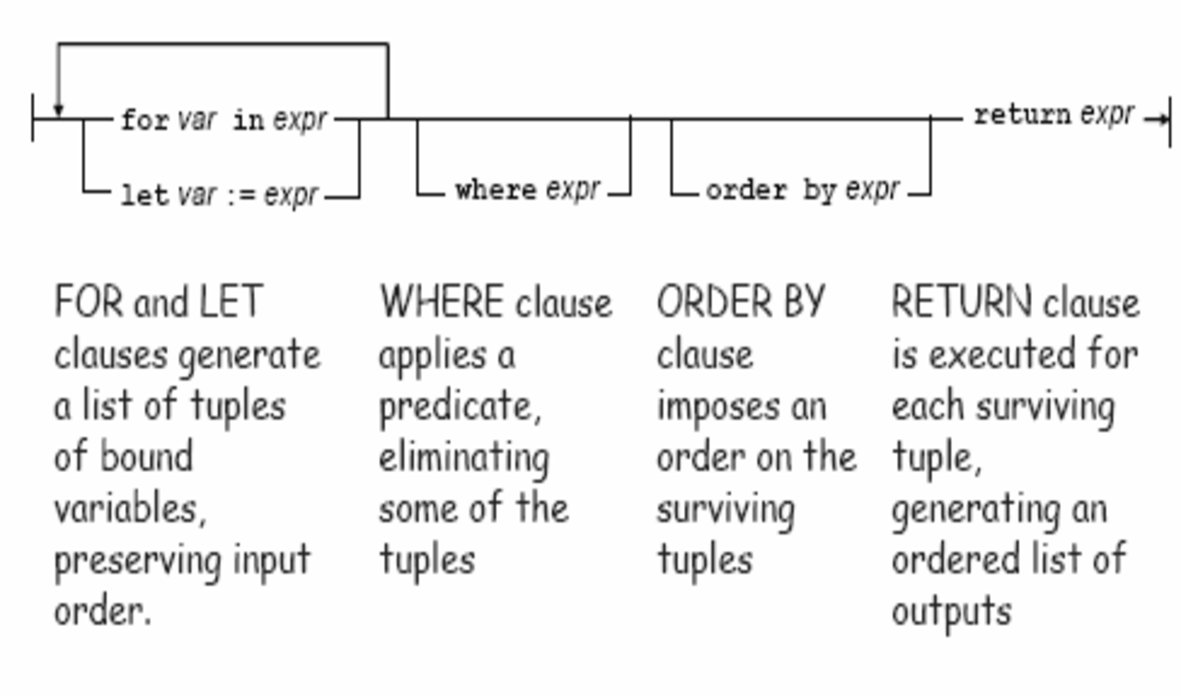
\includegraphics[scale=0.50]{flowr.pdf}
	\end{center}
\end{frame}

\begin{frame}[fragile]{\texttt{return} Statements}
\small
\begin{block}{The \texttt{return} Statement}
\begin{semiverbatim}
return \textit{XQuery\_expression}
\end{semiverbatim}
\end{block}
\normalsize
\begin{itemize}
	\item The \texttt{return} statement will return the sequence of elements represented by the XQuery expression
	\item A \texttt{return} statement is mandatory in every XQuery expression
\end{itemize}
\end{frame}

\begin{frame}[fragile]{\texttt{return} Statements}
\small
\begin{block}{The \texttt{return} Statement}
\begin{verbatim}
let $x := doc("library.xml")
return $x//lname
\end{verbatim}
\end{block}
\normalsize
\begin{itemize}
	\item The above statement will return all \texttt{<lname>} elements
\end{itemize}
\end{frame}

\begin{frame}[fragile]{\texttt{let} Statements}
\small
\begin{block}{The \texttt{let} Statement}
\begin{semiverbatim}
let \textit{variable} := \textit{XQuery\_expression}
\end{semiverbatim}
\end{block}
\normalsize
\begin{itemize}
	\item The \texttt{let} statement will assign to a variable the sequence of items described by an XQuery expression
\end{itemize}
\end{frame}

\begin{frame}[fragile]{\texttt{let} Statements}
\small
\begin{block}{The \texttt{let} Statement}
\begin{verbatim}
let $x := doc("company.xml")//lname
return $x
\end{verbatim}
\end{block}
\normalsize
\begin{itemize}
	\item The above statement will assign to \texttt{\$x} the \textit{sequence} of all \texttt{<lname>} elements
	\item The \texttt{return} statement will return that sequence
\end{itemize}
\end{frame}

\begin{frame}[fragile]{\texttt{let} Statements}
\small
\begin{block}{The \texttt{let} Statement}
\begin{verbatim}
let $x := doc("company.xml")//dep_name
return data($x/../../../lname)
\end{verbatim}
\end{block}
\normalsize
\begin{itemize}
	\item Even though we select nodes at one level, we still have access to the parent nodes
\end{itemize}
\end{frame}

\begin{frame}[fragile]{\texttt{for} Statements}
\small
\begin{block}{The \texttt{for} Statement}
\begin{semiverbatim}
for \textit{variable} in \textit{XQuery\_expression}
\end{semiverbatim}
\end{block}
\normalsize
\begin{itemize}
	\item A \texttt{for} statement will cause a variable to iterate through all the elements in the sequence of elements returned by an XQuery expression.
\end{itemize}
\end{frame}

\begin{frame}[fragile]{\texttt{for} Statements}
\small
\begin{block}{The \texttt{for} Statement}
\begin{verbatim}
for $x in doc("company.xml")//lname
return $x
\end{verbatim}
\end{block}
\normalsize
\begin{itemize}
	\item The above \texttt{for} statement will iterate through the sequence of \texttt{<lname>} elements
	\item The \texttt{return} statement will return each element individually (not as a sequence)
\end{itemize}
\end{frame}

\begin{frame}[fragile]{\texttt{for} Statements}
\small
\begin{block}{\texttt{for} vs. \texttt{let}}
\begin{verbatim}
for $x in doc("company.xml")//dep_name
return data($x/../../../lname)
\end{verbatim}
\end{block}
\normalsize
\begin{itemize}
	\item How does this query differ from a very similar earlier query that used \texttt{let}?
\end{itemize}
\end{frame}

\begin{frame}[fragile]{\texttt{for} vs. \texttt{let}}
\begin{itemize}
	\item In a \emph{for} statement, the variable iterates through the sequence of elements, \emph{one at a time}
	\item In a \emph{let} statement, the variable is assigned the \emph{entire sequence}
\end{itemize}
\end{frame}

\begin{frame}[fragile]{\texttt{for} Statements}
\small
\begin{block}{The \texttt{for} Statement}
\begin{verbatim}
for $x in doc("company.xml")//employee
let $y := $x/salary
return data($y)
\end{verbatim}
\end{block}
\normalsize
\begin{itemize}
	\item The above \texttt{for} statement will iterate through the sequence of \texttt{<employee>} elements and select the salary of each employee
\end{itemize}
\end{frame}

\begin{frame}[fragile]{\texttt{where} Statements}
\small
\begin{block}{The \texttt{where} Statement}
\begin{semiverbatim}
where \textit{predicate}
\end{semiverbatim}
\end{block}
\normalsize
\begin{itemize}
	\item The \texttt{where} clause may involve another XQuery expression
	\item It will filter out all elements that do not satisfy the predicate
\end{itemize}
\end{frame}

\begin{frame}[fragile]{\texttt{where} Statements}
\small
\begin{block}{The \texttt{where} Statement}
\begin{verbatim}
for $x in doc("company.xml")//employee
where $x/salary > 60000
return $x
\end{verbatim}
\end{block}
\normalsize
\begin{itemize}
	\item In a \texttt{for} loop, the predicate is applied to each of the values of the loop variable
	\item The \texttt{for} loop will skip those values of the loop variable that do not satisfy the predicate
	\item The above query will return the employee elements of all employees making more than \$60,000
\end{itemize}
\end{frame}

\begin{frame}[fragile]{\texttt{where} Statements}
\small
\begin{block}{The \texttt{where} Statement}
\begin{verbatim}
let $x := doc("company.xml")//employee
where $x/salary > 60000
return $x
\end{verbatim}
\end{block}
\normalsize
\begin{itemize}
	\item Outside of a \texttt{for} loop, the values of the variable are not iterated, but are treated as one sequence
	\item The predicate is applied to the entire sequence
	\item The above query will return \textit{all} employee elements because there is at least one who makes more than \$60,000
\end{itemize}
\end{frame}

\begin{frame}[fragile]{\texttt{where} Statements}
\small
\begin{block}{\texttt{where} vs. an XPath Predicate}
\begin{verbatim}
for $x in doc("company.xml")//employee[salary > 60000]
return $x
\end{verbatim}
\end{block}
\normalsize
\begin{itemize}
	\item In this example, the variable iterates through only the employees who make more than \$60,000
\end{itemize}
\end{frame}

\begin{frame}[fragile]{\texttt{where} Statements}
\small
\begin{block}{\texttt{where} vs. an XPath Predicate}
\begin{verbatim}
let $x := doc("company.xml")//employee[salary > 60000]
return $x
\end{verbatim}
\end{block}
\normalsize
\begin{itemize}
	\item In this example, the variable is assigned the sequence of elements consisting only of the employees who make more than \$60,000
\end{itemize}
\end{frame}

% \begin{frame}[fragile]{\texttt{for} vs. \texttt{let}}
% \small
% \begin{block}{\texttt{for} vs. \texttt{let}}
% \begin{verbatim}
% for $x in doc("company.xml")//dep_name
% return data($x/../../../lname)
% \end{verbatim}
% \end{block}
% \normalsize
% \begin{itemize}
% 	\item How does this query differ from a very similar earlier query that used \texttt{let}?
% \end{itemize}
% \end{frame}

\begin{frame}[fragile]{\texttt{order by} Statements}
\small
\begin{block}{The \texttt{order by} Statement}
\begin{semiverbatim}
order by \textit{XQuery\_expression}
\end{semiverbatim}
\end{block}
\normalsize
\begin{itemize}
	\item The \texttt{order by} clause will arrange the elements of a variable into a specified order
	\item The XQuery expression must take on one value per item being sorted
\end{itemize}
\end{frame}

\begin{frame}[fragile]{\texttt{order by} Statements}
\small
\begin{block}{The \texttt{order by} Statement}
\begin{verbatim}
for $x in doc("company.xml")//employee
order by $x/gender
return data($x/fname)
\end{verbatim}
\end{block}
\normalsize
\begin{itemize}
	\item The above expression will return the first names of the employees, with the females first and then the males
\end{itemize}
\end{frame}

\begin{frame}[fragile]{\texttt{order by} Statements}
\small
\begin{block}{Order by Multiple Fields}
\begin{verbatim}
for $x in doc("company.xml")//employee
order by $x/gender, $x/lname
return data($x/concat(fname, " ", lname, ","))
\end{verbatim}
\end{block}
\normalsize
\begin{itemize}
	\item The above expression will return the full names, with the females first and then the males, each group alphabetized by last name
\end{itemize}
\end{frame}

\begin{frame}[fragile]{\texttt{order by} Statements}
\small
\begin{block}{Descending Order}
\begin{verbatim}
for $x in doc("company.xml")//employee
order by count($x/*/dependent) descending
return data($x/concat(fname, " ", lname, ","))
\end{verbatim}
\end{block}
\normalsize
\begin{itemize}
	\item The above expression will list the names of the employees, sorted in descending order by the number of dependents
\end{itemize}
\end{frame}

\begin{frame}[fragile]{\texttt{order by} Statements}
\small
\begin{block}{Missing Elements}
\begin{verbatim}
for $x in doc("library.xml")//collection
order by $x/authors/author/lname
return data($x/title)
\end{verbatim}
\end{block}
\normalsize
\begin{itemize}
	\item The collections without authors would be listed first
\end{itemize}
\end{frame}

\begin{frame}[fragile]{\texttt{order by} Statements}
\small
\begin{block}{Missing Elements}
\begin{verbatim}
empty greatest
empty least
\end{verbatim}
\end{block}
\normalsize
\begin{itemize}
	\item We may append \emph{\tt empty greatest} or \emph{\tt empty least} to the \emph{\tt order by} clause
	\item The default is \emph{\tt empty least}
\end{itemize}
\end{frame}

\begin{frame}[fragile]{\texttt{order by} Statements}
\small
\begin{block}{Missing Elements}
\begin{verbatim}
for $x in doc("library.xml")//collection
order by $x/authors/author/lname empty greatest
return data($x/title)
\end{verbatim}
\end{block}
\normalsize
\begin{itemize}
	\item Now, collections with the author name would be listed first
\end{itemize}
\end{frame}

\section{Constructors}

\begin{frame}[fragile]{Direct Constructors}
\small
\begin{block}{Direct Constructors}
\begin{verbatim}
<lname>Twain</lname>
\end{verbatim}
\end{block}
\normalsize
\begin{itemize}
	\item An element may be constructed using a \emph{direct constructor}
	\item For example, the above expression will construct an \texttt{<lname>} element
\end{itemize}
\end{frame}

\begin{frame}[fragile]{Direct Constructors}
\small
\begin{block}{Nested Constructors}
\begin{verbatim}
<employee><lname>Twain</lname></employee>
\end{verbatim}
\end{block}
\normalsize
\begin{itemize}
	\item An element constructor may contain properly nested element constructors
	\item For example, the above expression will construct an \texttt{lname} element embedded within an \texttt{employee} element
\end{itemize}
\end{frame}

\begin{frame}[fragile]{Direct Constructors}
\small
\begin{block}{XQuery Expressions within Constructors}
\begin{verbatim}
<lname>$emp/lname</lname>
<lname>{$emp/lname}</lname>
\end{verbatim}
\end{block}
\normalsize
\begin{itemize}
	\item The content of the constructor is interpreted literally unless it is enclosed within curly braces.
	\item The first example above will construct an\texttt{ <lname>} element containing the text \texttt{\$emp/lname}.
	\item The second example will construct an \texttt{<lname>} element with the value of \texttt{\$emp/lname} substituted in.
\end{itemize}
\end{frame}

\begin{frame}[fragile]{Direct Constructors}
\small
\begin{block}{XQuery Expressions within Constructors}
\begin{verbatim}
<name>{data($emp/lname)}</name>
\end{verbatim}
\end{block}
\normalsize
\begin{itemize}
	\item We may use the \texttt{data()} function to strip the tags from the element.
	\item The above example receives an \texttt{<lname>} element and produces a \texttt{<name>} element with the same value.
\end{itemize}
\end{frame}

\begin{frame}[fragile]{Direct Constructors}
\small
\begin{block}{Direct Constructors}
\scriptsize
\begin{verbatim}
<html>
 <body>
  <h2>List of Employees</h2>
  <ul>
  {
    for $name in doc("company.xml")//employee/lname
    return <li>{data($name)}</li>
  }
  </ul>
 </body>
</html>
\end{verbatim}
\end{block}
\normalsize
\begin{itemize}
	\item The above expression will create an HTML list of employee's last names.
	\item Note the use of the braces within the \texttt{<li>} constructor as well as the braces within the \texttt{<ul>} constructor.
	\item The value of the XQuery expression must represent a single XML element (with properly nested subelements).
\end{itemize}
\end{frame}

\begin{frame}[fragile]{Computed Constructors}
\small
\begin{block}{Computed Constructors}
\begin{semiverbatim}
element \emph{element_name} {\emph{contents}}
\end{semiverbatim}
\end{block}
\normalsize
\begin{itemize}
	\item Instead of a direct constructor, we may use a \alert{computed constructor}.
\end{itemize}
\end{frame}

\begin{frame}[fragile]{Computed Constructors}
\small
\begin{block}{Computed Constructors}
\begin{verbatim}
element html {
  element body {
    element h2 {"List of Employees"},
    element ul {
        for $lname in doc("company.xml")//lname
        return element li {data($lname)}
    }
  }
}
\end{verbatim}
\end{block}
\normalsize
\begin{itemize}
	\item The previous example could be written like this.
\end{itemize}
\end{frame}

\begin{frame}[fragile]{Computed Constructors}
\small
\begin{block}{Variable Element Name}
\begin{verbatim}
element employee
{
    for $x in doc("company.xml")//lname
    return element {data($x/name(..))} {data($x)}
}
\end{verbatim}
\end{block}
\normalsize
\begin{itemize}
	\item The above example will create \texttt{<employee>} elements.
\end{itemize}
\end{frame}

\begin{frame}[fragile]{Comment Constructors}
\small
\begin{block}{Comment Constructor}
\begin{verbatim}
comment {"Hello, world"}
\end{verbatim}
\end{block}
\normalsize
\begin{itemize}
	\item The comment constructor will create a comment element.
	\item This example creates \texttt{<!$--$Hello, world$--$>}.
\end{itemize}
\end{frame}

\begin{frame}[fragile]{Constructed Attributes}
\small
\begin{block}{Attribute Constructor}
\begin{semiverbatim}
<\textit{element_name}>
    \textit{value} {attribute \textit{attr_name} \textit{attr_val}}
</\textit{element_name}>
\end{semiverbatim}
\end{block}
\normalsize
\begin{itemize}
	\item An attribute of an element can be constructed.
\end{itemize}
\end{frame}

\begin{frame}[fragile]{Constructed Attributes}
\small
\begin{block}{title}
\begin{verbatim}
<greeting> 
 { attribute whom {"World"}, "Hello" }
</greeting>
\end{verbatim}
\end{block}
\normalsize
\begin{itemize}
	\item The above example creates the element \begin{center}\texttt{$<$greeting whom="world"$>$ Hello $<$/greeting$>$}\end{center}
\end{itemize}
\end{frame}

\begin{frame}[fragile]{Constructed Attributes}
\small
\begin{block}{title}
\begin{verbatim}
for $emp in doc("company.xml")//employee
let $elem := name($emp)
let $value := $emp/data(@empID)
let $attr := name($emp/@empID)
return 
 element {$attr} {attribute {$elem} {$value}, $emp/*}
\end{verbatim}
\end{block}
\normalsize
\begin{itemize}
	\item This example transforms \texttt{$<$employee empID="E1"$>$} into \texttt{$<$empID employee="E1"$>$}, etc.
\end{itemize}
\end{frame}

\section{Joins}

\begin{frame}[fragile]{Joins}
\begin{itemize}
	\item There is no join operator in XQuery
	\item Still, FLOWR statements can be used to create a join
	\item We use the predicate to match the elements
	\item XPath predicates can also be used to perform joins, although the FLOWR syntax is more convenient
\end{itemize}
\end{frame}

\begin{frame}[fragile]{Joins}
\small
\begin{block}{Joins}
\begin{verbatim}
for $book in doc("books.xml")//book ,
    $author in doc("authors.xml")//author
where $book/@authRefs = $author/@authID
return concat(data($book/title), " by ", 
    data($author/lname))
\end{verbatim}
\end{block}
\normalsize
\begin{itemize}
	\item This code will produce each title together with its author
	\item Note that the \texttt{for} statement uses two variables
	\item Note that the query combines content from two different XML sources
\end{itemize}
\end{frame}



\section{Extensions}

\begin{frame}[fragile]{Full-Text Search}
\begin{itemize}
\item XQuery and XPath Full Text Recommendation (XQFT) is an extension of the XQuery language
\item It can be used to both query XML documents and single strings for words and phrases.
\item Supports scoring models
\end{itemize}

\begin{block}{}
\begin{verbatim}
"This is YOUR World" contains text "your world"
\end{verbatim}
\end{block}

\begin{block}{}
\begin{verbatim}
for $text score $score in ("word1", "word1 word2")
where $text contains text "word1"
order by $score descending
return <hit score="{ $score }">{ $text }</hit>
\end{verbatim}
\end{block}

\end{frame}




\begin{frame}[fragile]{XQuery Update Facility}
\begin{itemize}
\item Convenient means of modifying XML documents or data
\item Transform expressions, plus a series of updating expressions with secondary effects
\end{itemize}

\begin{block}{}
\begin{verbatim}
let $node := <root><a/></root>
return update insert <b/> into $node/a
\end{verbatim}
\end{block}

\begin{block}{}
\begin{verbatim}
copy $c := //c[@id = 5]
modify (
  delete nodes $c/a/b,
  rename node $c as "not_c"
)
return $c
\end{verbatim}
\end{block}

\end{frame}

% ------------------------------------------------------------

\finalframe{Questions?}

\end{document}